\documentclass{../../bredelebeamer}
\usepackage{multirow}
\usepackage{pdfpages}
\usepackage{braket,bigstrut}
\usepackage{palatino}
\usepackage{multicol,bigstrut}
\usepackage{listings}
\usepackage{tikz,slashed}
\usepackage{pgfplots}
\pgfplotsset{compat=1.17}
\usepackage{booktabs}
\usepackage{amsmath,amssymb,amsfonts,cancel,physics,siunitx}
\usepackage{ragged2e}
\usetikzlibrary{positioning,shadows,backgrounds,calc}%
\setbeamercolor{footnote mark}{fg=black}
\setbeamercolor{footnote}{fg=black}


\renewcommand{\baselinestretch}{0.9}

\usepackage[backend=bibtex8,style=authortitle,autocite=footnote]{biblatex}
\addbibresource{references.bib}

\renewbibmacro*{cite:title}{%
	\printtext[bibhyperref]{%
		\printfield[citetitle]{labeltitle}%
		\setunit{\space}%
		\printtext[parens]{\printdate}%
	}%
}

\renewcommand{\figurename}{{\bf Fig.}}
\usefonttheme{serif} % default family is serif

\renewcommand{\baselinestretch}{0.9}

\title[Higgs-Portal DM with VBF at HL-LHC]{Probing Higgs-Portal Dark Matter with VBF Signatures at the HL-LHC}
\subtitle{}
\author[C. Rodríguez]{%
	\vspace{2em}\\
	PhD(c). Cristian Fernando Rodríguez Cruz\inst{1}\\
    $$ $$
    Asesor: Prof. Andrés Florez\inst{1}\\
	\vspace{1em}
}

\institute[Uniandes]{\inst{1} Universidad de los Andes\and
% \inst{2} Pontificia Universidad Católica del Perú 
}
\date{\today}
\lstset{language=C++,
  basicstyle=\ttfamily,
  keywordstyle=\color{blue}\ttfamily,
  stringstyle=\color{red}\ttfamily,
  commentstyle=\color{green}\ttfamily,
  morecomment=[l][\color{magenta}]{\#}
}

\begin{document}
\begin{frame}
    \titlepage
\end{frame}
\begin{frame}{Abstract}
    \justifying
    We investigate current and projected constraints on Higgs-portal dark matter (DM) models, focusing on both scalar and fermionic DM candidates, using vector boson fusion (VBF) production of the Higgs boson at the LHC. By analyzing the parameter space in the plane of DM mass versus the Higgs-DM coupling, we aim to reinterpret existing LHC VBF + MET searches to set bounds on the invisible Higgs decay channels.

    \vfill

    To this end, we perform simulations in MadGraph5\_aMC@NLO under LHC conditions to compute cross sections for VBF Higgs production followed by invisible decays. Experimental efficiencies are estimated through a recast of public analyses targeting the process $pp \to jj + \text{MET}$. We then rescale the integrated luminosity to project the reach of the High-Luminosity LHC (HL-LHC), identifying both currently excluded regions and those potentially probed with 3 ab$^{-1}$. Our results provide updated exclusion contours and projections in the Higgs-portal to DM parameter space.
\end{frame}

\begin{frame}{Outline}
    \tableofcontents
\end{frame}

\section{Introduction}
\begin{frame}{Dark Matter: A Missing Piece}{One of the Main Problems in 
Contemporary Physics}
    
    \begin{columns}[T]
        \begin{column}{0.53\textwidth}
            \textbf{Key Properties:}
            \begin{itemize}
                \item \textbf{26\%} of universe's energy density (Planck 2018)
                \item \textbf{Cold \& non-relativistic} ($\Rightarrow$ structure formation)
                \item \textbf{Weakly interacting}: No EM/strong forces
                \item \textbf{Invisible}: Only gravitational evidence
                %\item The interaction comunicates the SM with the DM sector.
            \end{itemize}
        \end{column}
        \begin{column}{0.45\textwidth}
            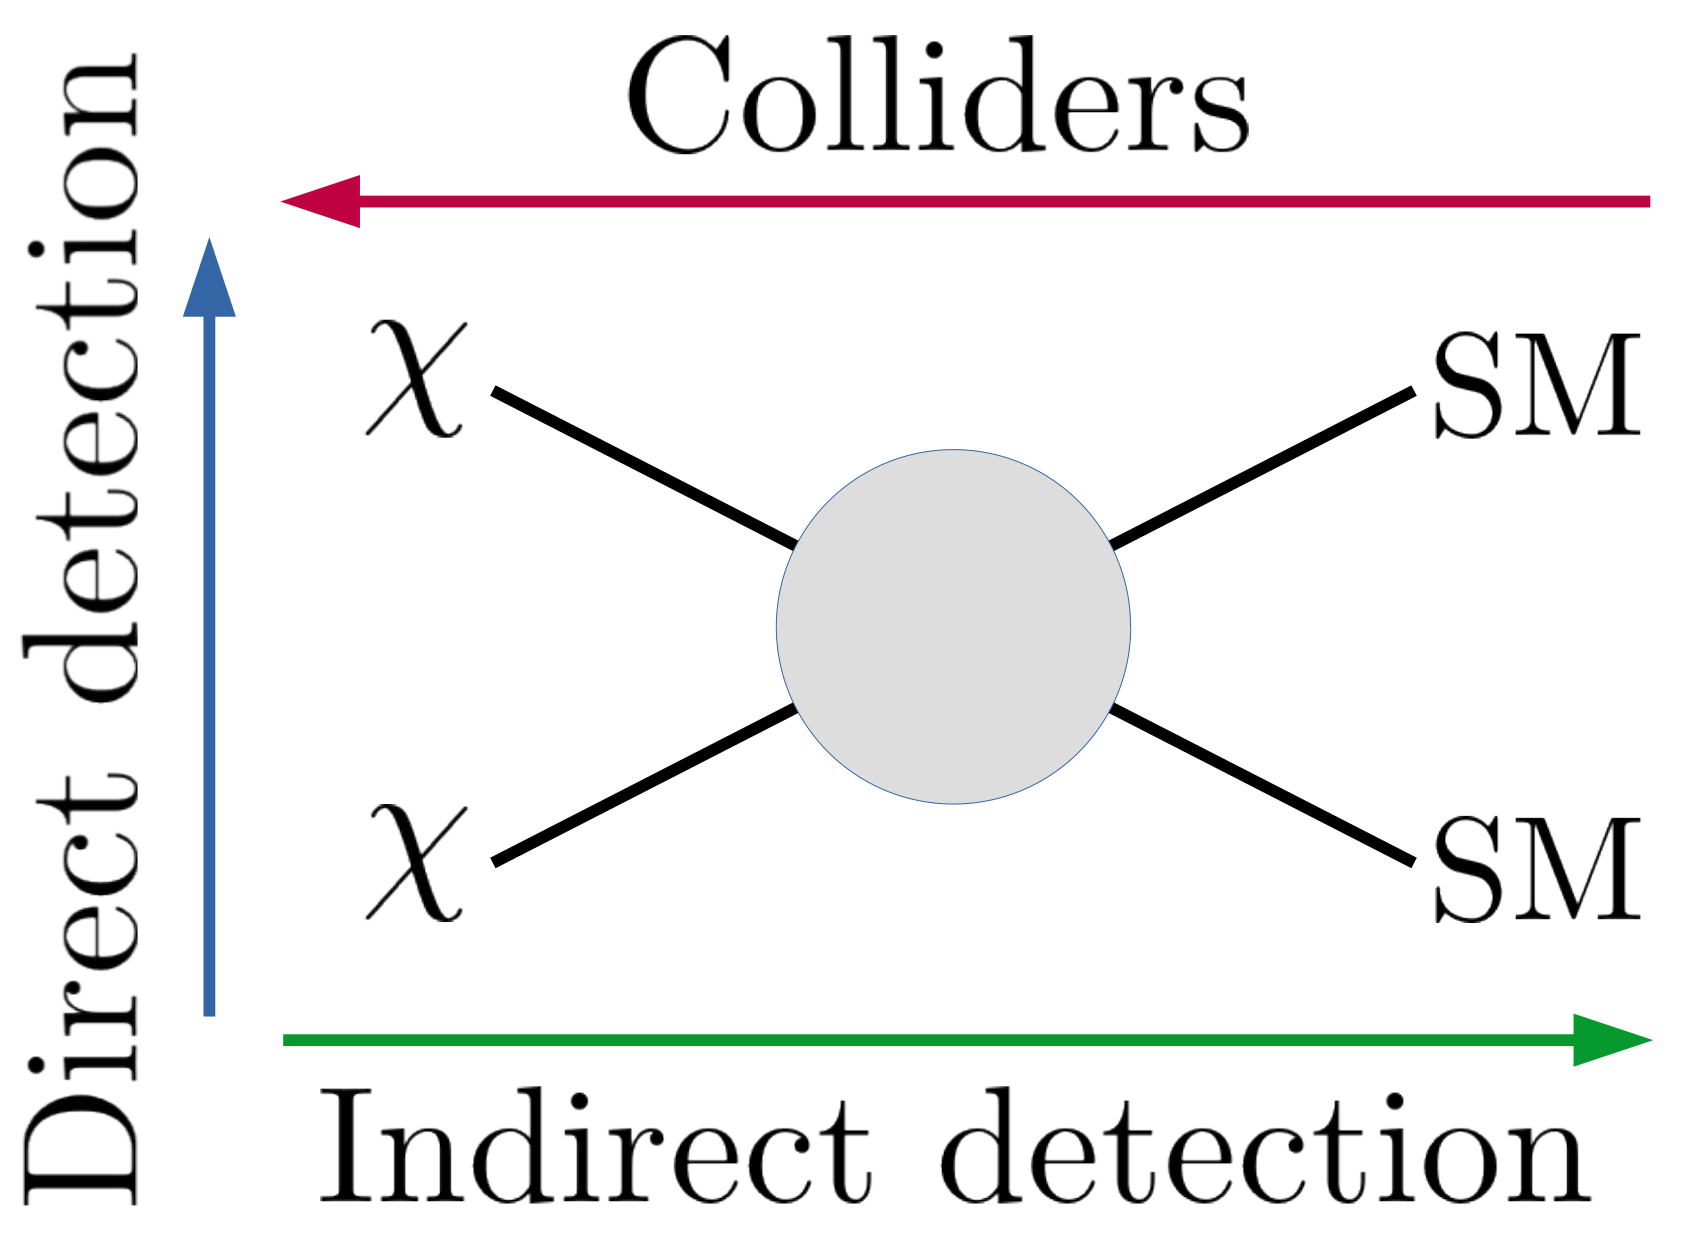
\includegraphics[width=\textwidth]{../Images/schematic_DMdetections.png}
        \end{column}
    \end{columns}

    \vspace{0.5cm}
    \pause

    \textbf{The Higgs Portal Advantage:}
    \begin{center}
        
\includegraphics[width=0.6\textwidth]{../Images/Higgs_portal.png} \\
        \footnotesize Simplest SM-DM connection via Higgs boson (spin-0 mediator)
    \end{center}
\end{frame}

\begin{frame}{Higgs $\to$ invisible: a window to new physics}
  \begin{itemize}
    \item In the Standard Model (SM), the Higgs is a fundamental scalar with $m_H = 125.1$~GeV and $\Gamma_H^{\text{SM}} \approx 4.07$ MeV.
    \vfill
    \item The current measurement of the total Higgs width is $\Gamma_H = 3.7^{+1.9}_{-1.4}$ MeV,\\ $\Rightarrow$ \textbf{there is still window for non-SM contributions.}
    \vfill
    \item In SM extensions, the Higgs can couple to the dark sector with a sizable fraction:
    \[
      \text{BR}(H \to \text{inv}) = \frac{\Gamma_H^{\text{inv}}}{\Gamma_H^{\text{SM}} + \Gamma_H^{\text{inv}}}
    \]
    
    \item Experimental limit from VBF + MET:
    \[
      \text{BR}(H \to \text{inv}) < 0.145
    \]
    \vfill
    \item  \textbf{Invisible Higgs decays offer a window to explore new physics and hint at the presence of dark particles.}
  \end{itemize}
\end{frame}

\begin{frame}{Vector Boson Fusion (VBF) Production}

    One of the most studied and well known production mechanisms of the Higgs boson at the LHC is VBF. 
    
    \vfill 

    In proton-proton collisions, the quark components of the protons interact via the exchange of vector bosons (W or Z), leading to the production of a Higgs boson in association with two forward jets.

    \vfill 

    The Higgs boson is narrow, so the total cross section can be approximated as production cross section times the branching ratio to invisible decays
    \begin{equation*}
            \Gamma_h/m_h \sim 3 \times 10^{-5}
            \quad\Longrightarrow\quad
            \sigma_{\text{total}} \approx \sigma_{\text{prod}} (\textcolor{red}{pp\boldsymbol{\to}j\,j\, h})  \times \text{BR}(\textcolor{blue}{h \boldsymbol{\to} \text{inv.}})
    \end{equation*}

    \begin{minipage}{0.42\textwidth}
        \begin{center}
            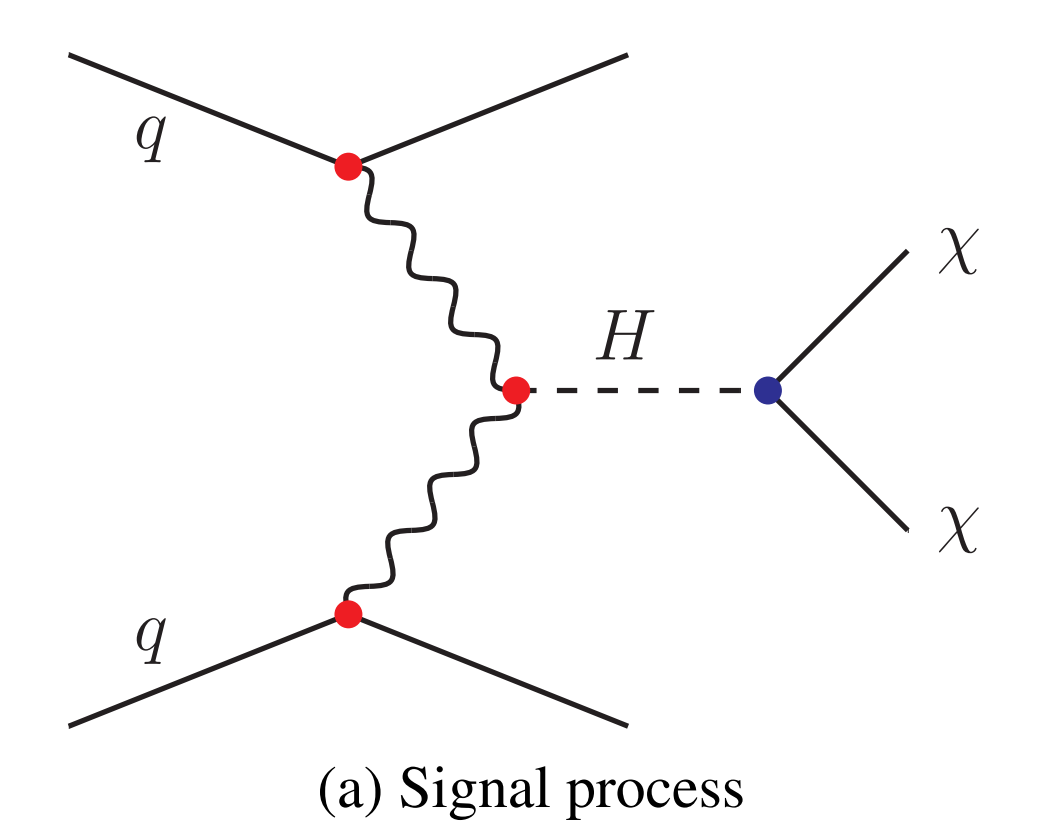
\includegraphics[width=\textwidth]{../Images/VBF.png}
        \end{center}
    \end{minipage}
    \hfill
    \begin{minipage}{0.5\textwidth}
        \begin{itemize}
            \item This process is characterized by the exchange of two vector bosons in t-channel that produces a Higgs boson in association with two jets. 
            \vspace{0.5cm}
            \item The Higgs to invisible decay channel could be characterized by the lost momentum in a detector in the final state.
        \end{itemize}
        

    \end{minipage}
\end{frame}

\section{Monte Carlo Method}
\begin{frame}{Monte Carlo Method Workflow}
	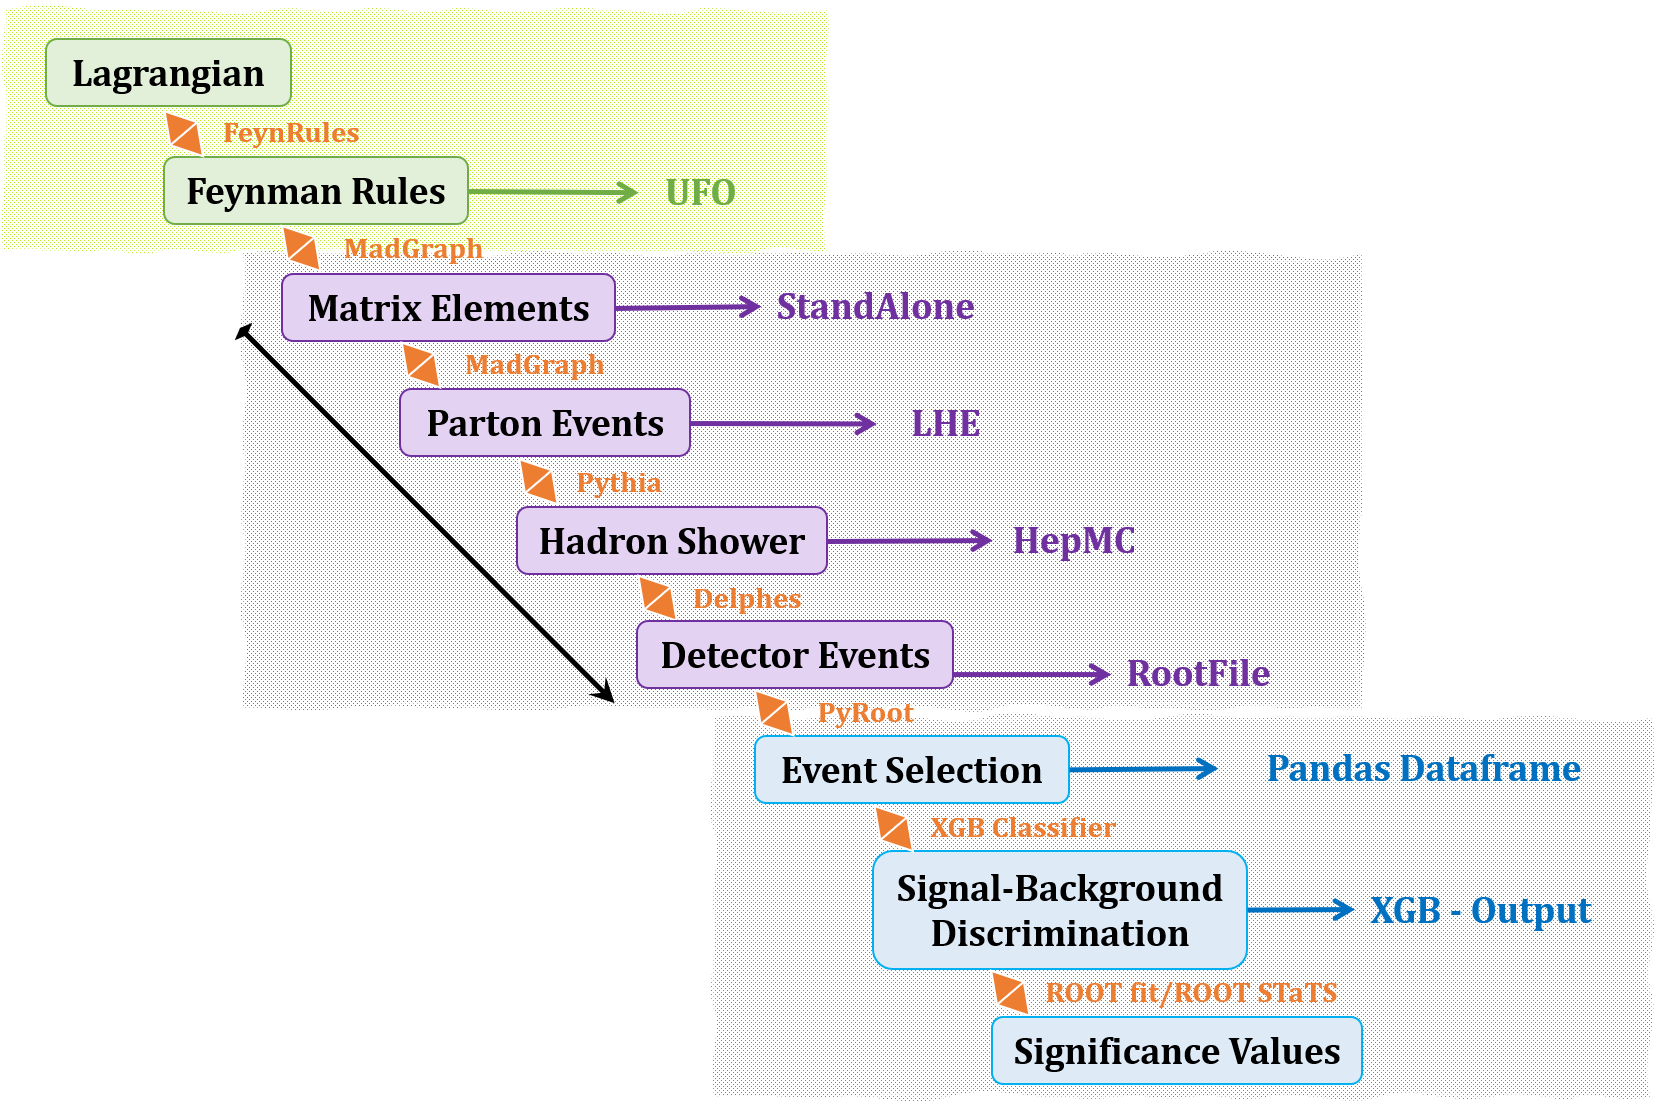
\includegraphics[width=1.0\linewidth]{../Images/Workflow.png}
\end{frame}

\begin{frame}{Madgraph-Pythia8-Delphes for Colliders}
	\begin{center}
		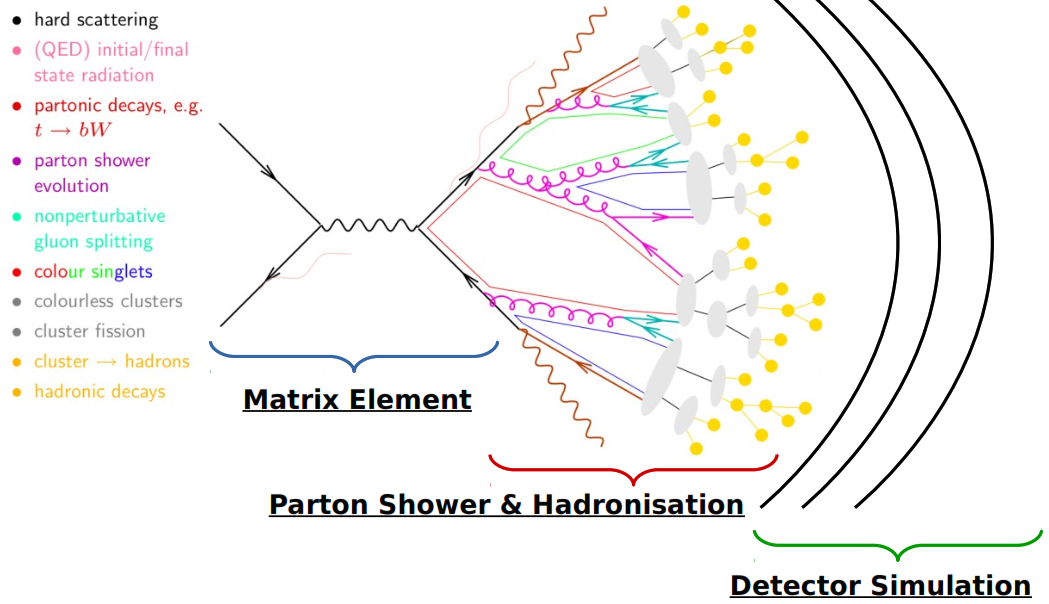
\includegraphics[width=.99\linewidth]{../Images/Madgraph.png}
	\end{center}
\end{frame}

\section{Observables}
\begin{frame}{Kinematic Variables}
    From Spherical coordinates,
    $$
    \begin{cases}
        \text{Pseudorapidity: } \eta = -\ln\tan(\theta/2) \\
        \text{Transverse momentum: } p_T = p \sin(\theta) \\
        \text{Azimuthal angle: } \phi\\
        \text{Deposited energy: } E \\
    \end{cases}
    $$

	\begin{center}
		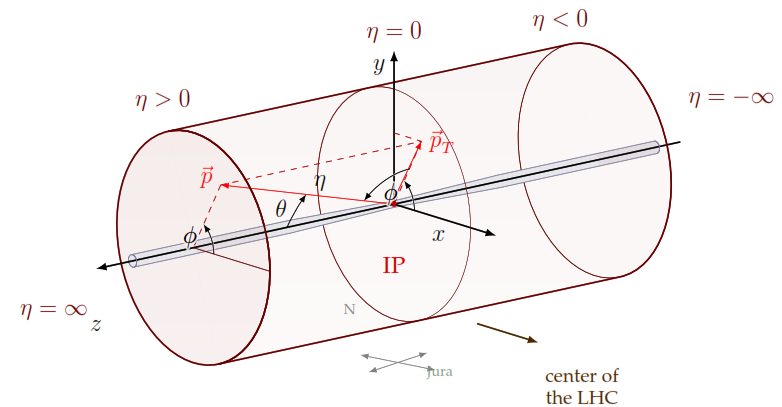
\includegraphics[width=.98\linewidth]{../Images/Kinematic_Variables.png}
	\end{center}
\end{frame}

\begin{frame}{Example of a VBF + MET Event in the CMS Detector}
    There is not initial momentum in the transverse plane, so from the conservation of momentum, we define the missing transverse momentum as
    $$
        \va*{p}_T^{\text{ mis}} = - \sum_{i} \va*{p}_{T,i}^{\text{ vis}}
    $$
    \begin{center}
        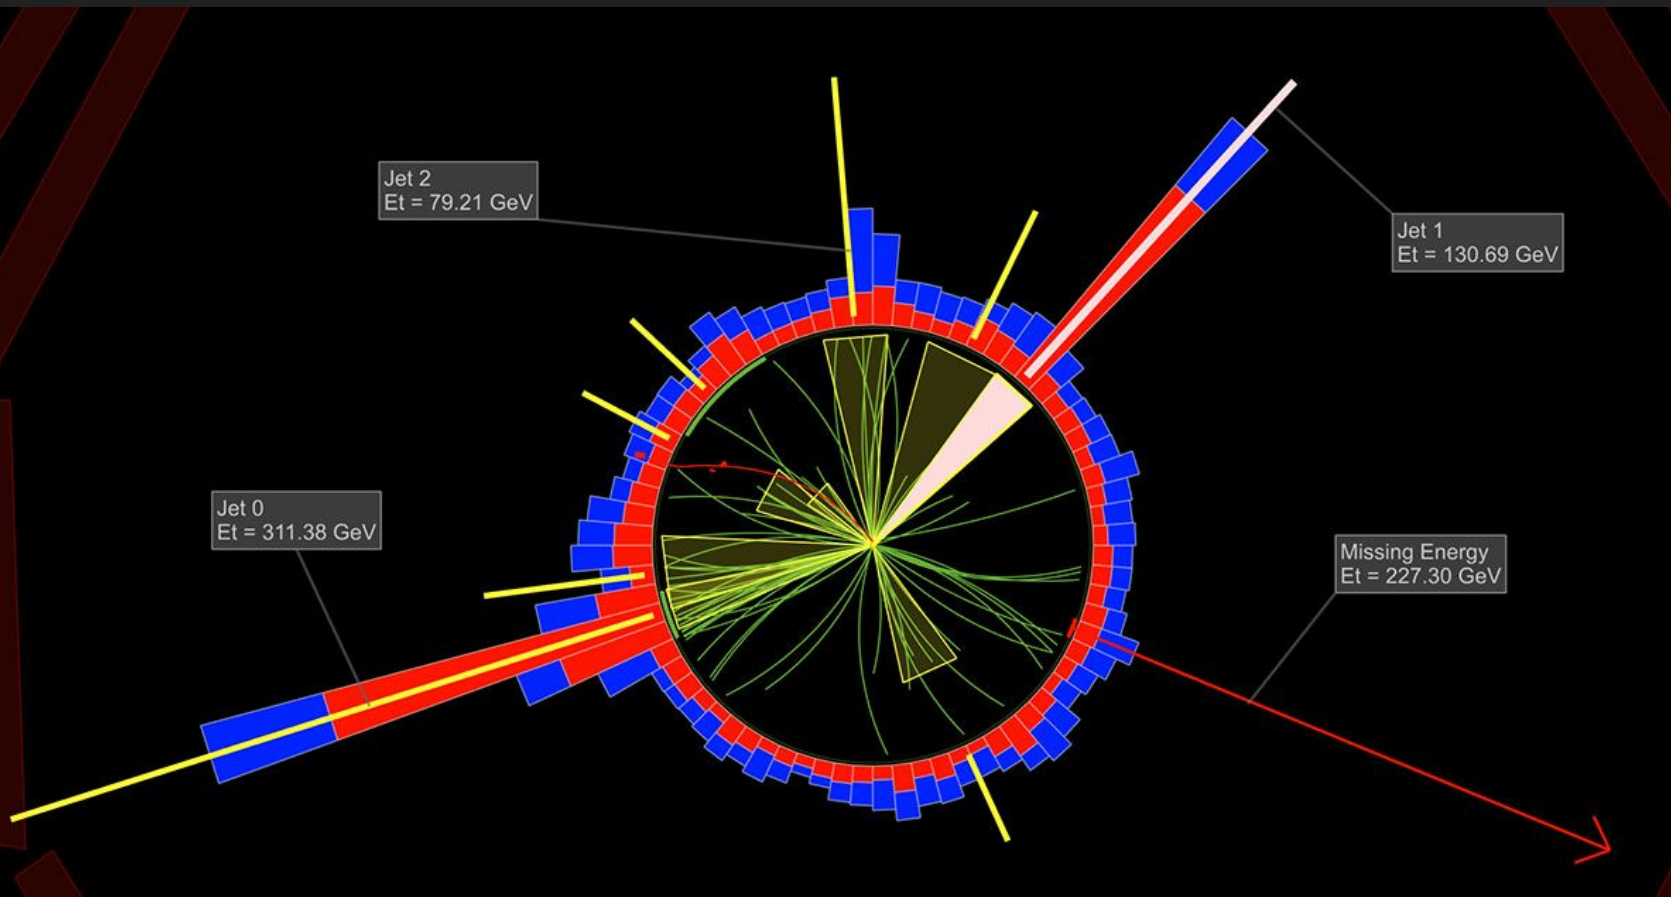
\includegraphics[width=.90\linewidth]{../Images/real_vbf_event.png}
    \end{center}
\end{frame}


\section{VBF Kinematics}
\begin{frame}{Current Results from VBF + MET Searches}
    \begin{columns}
        \begin{column}{0.4\textwidth}
            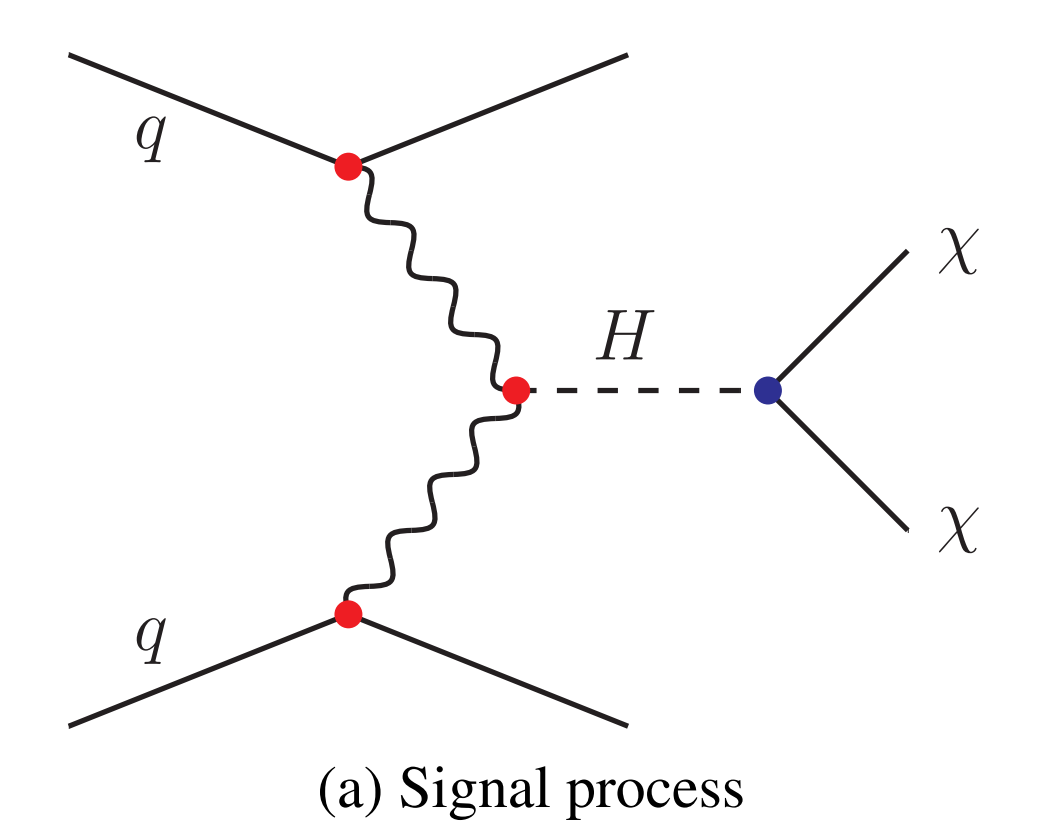
\includegraphics[width=\textwidth]{../Images/VBF.png}
        \end{column}
        \begin{column}{0.6\textwidth}
            Based on Criteria from 
            \begin{itemize}
                \item CMS: \cite{CMS:2022qva}
                \item ATLAS:\cite{ATLAS:2022yvh}
            \end{itemize}
        \end{column}
    \end{columns}
    Some basic criteria must to be satisfied to \textbf{preselect} the events:
    \begin{itemize}
        \item 0 electrons
        \item 0 muons
        \item 0 isolated photons
        \item At least 2 jets with $p_T > 30$ GeV
        \item Large missing transverse momentum ($p_T^{\text{miss}} > 100$ GeV)
    \end{itemize}

    % \begin{minipage}{0.47\textwidth}
    %     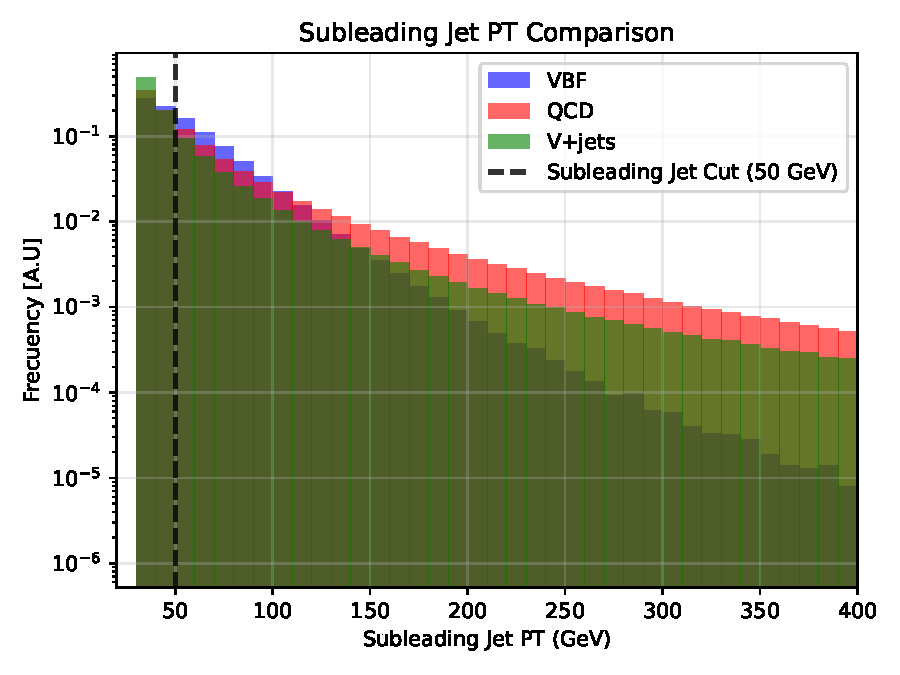
\includegraphics[width=\textwidth]{../Images/subleading_jet_pt_comparison.pdf}
    % \end{minipage}
\end{frame}
\begin{frame}{VBF Jets are boosted with High-PT signatures}{Leading Jet}
    \begin{minipage}{0.97\textwidth}
        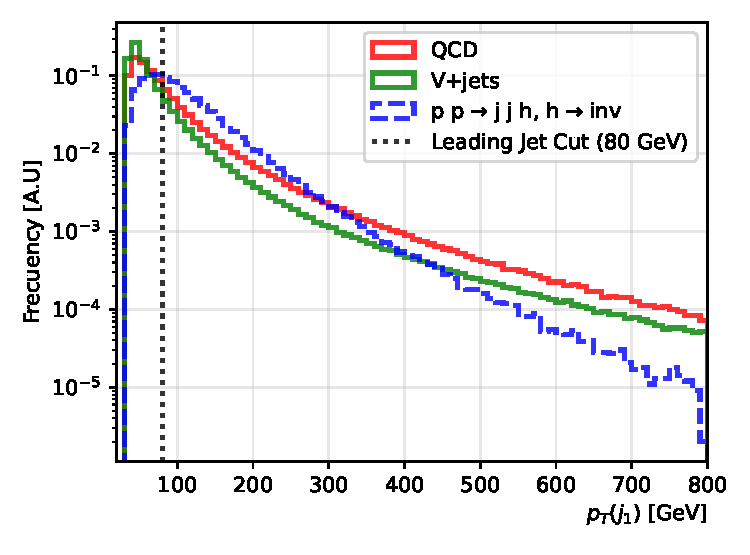
\includegraphics[width=\textwidth]{../Images/leading_jet_pt_comparison.pdf}
    \end{minipage}
\end{frame}

\begin{frame}{VBF Jets are boosted with High-PT signatures}{Subleading Jet}
    \begin{minipage}{0.97\textwidth}
        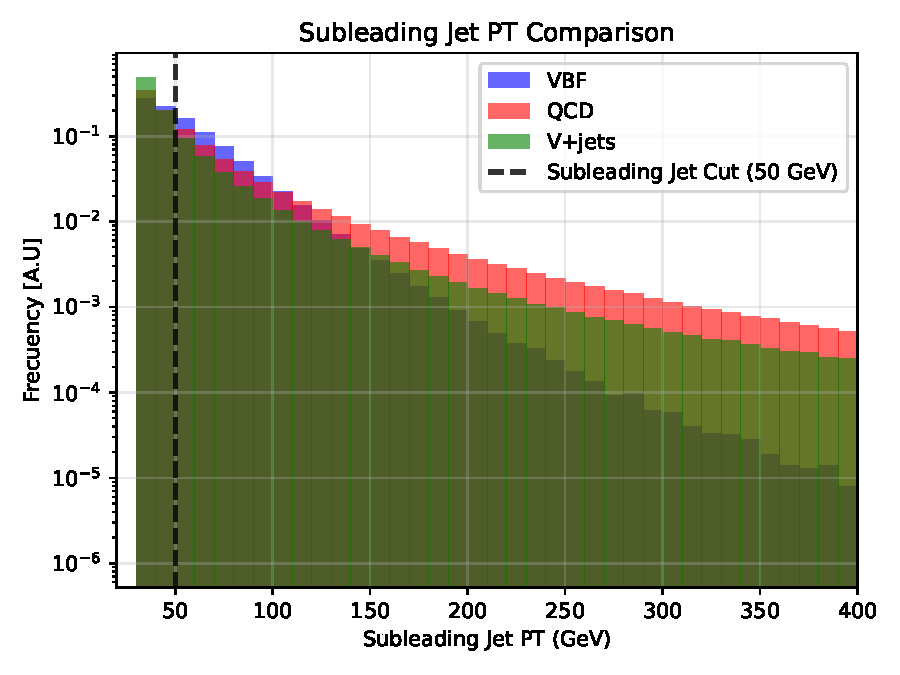
\includegraphics[width=\textwidth]{../Images/subleading_jet_pt_comparison.pdf}
    \end{minipage}
\end{frame}
\begin{frame}{VBF Jets are forward}
    \begin{minipage}{0.97\textwidth}
        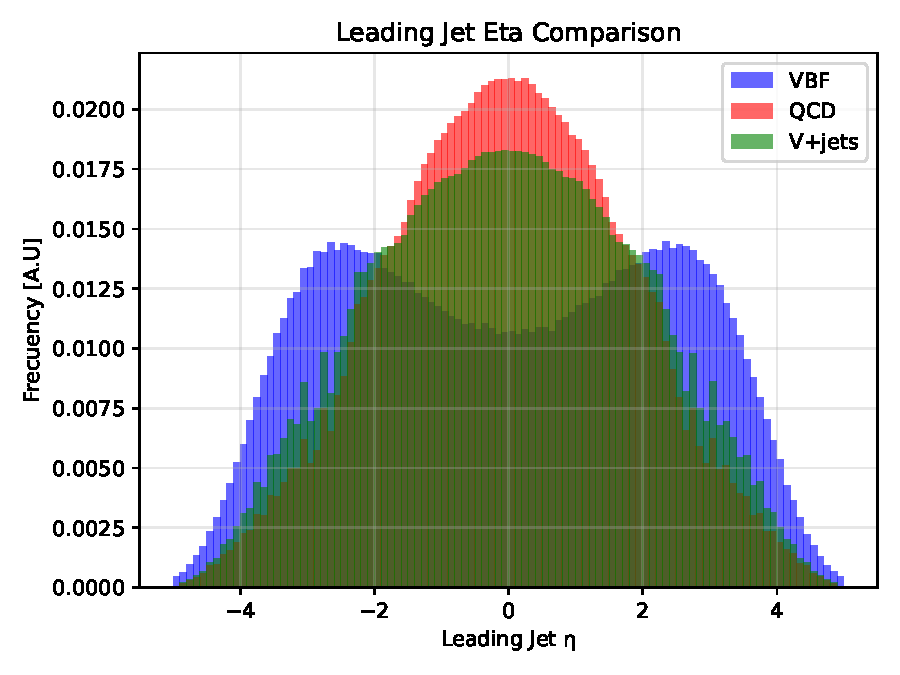
\includegraphics[width=\textwidth]{../Images/leading_jet_eta_comparison.pdf}
    \end{minipage}
    % \begin{minipage}{0.47\textwidth}
    %     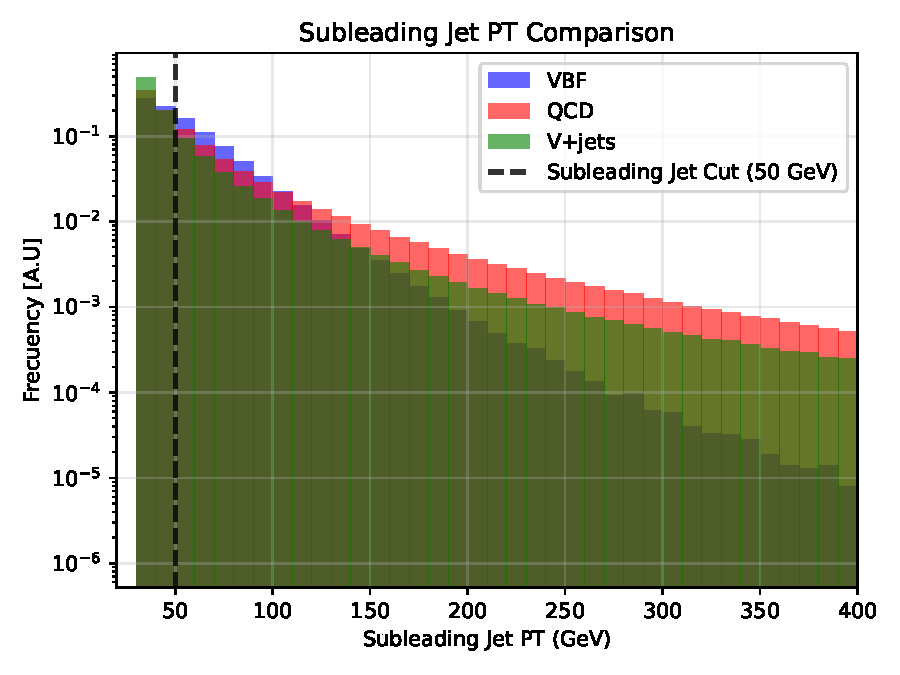
\includegraphics[width=\textwidth]{../Images/subleading_jet_pt_comparison.pdf}
    % \end{minipage}
\end{frame}

\begin{frame}{VBF Jets are in opposite longitudinal hemispheres}
    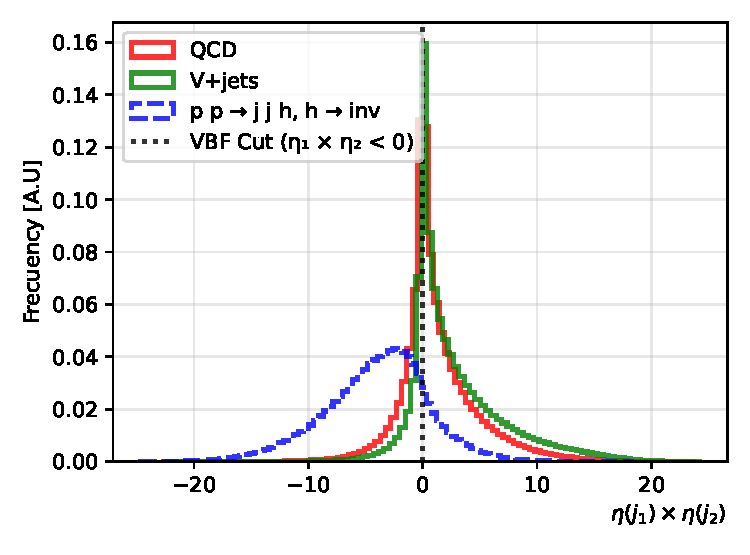
\includegraphics[width=\textwidth]{../Images/eta_product_comparison.pdf}
\end{frame}

\begin{frame}{VBF Jets have a large Delta-$\eta$ separation}
    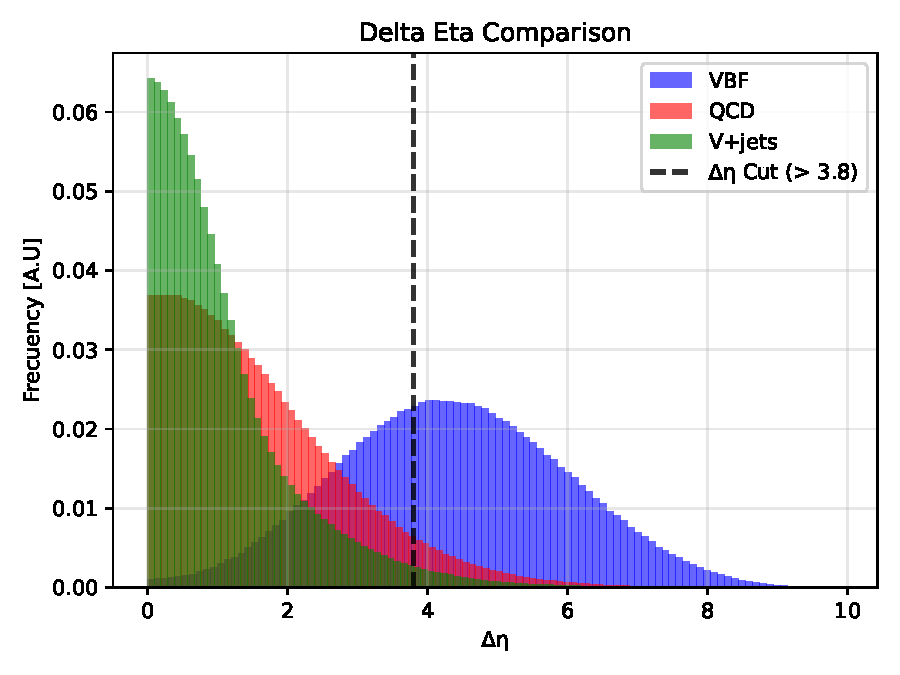
\includegraphics[width=\textwidth]{../Images/delta_eta_comparison.pdf}
\end{frame}
\begin{frame}{VBF Jets are not back-to-back}
    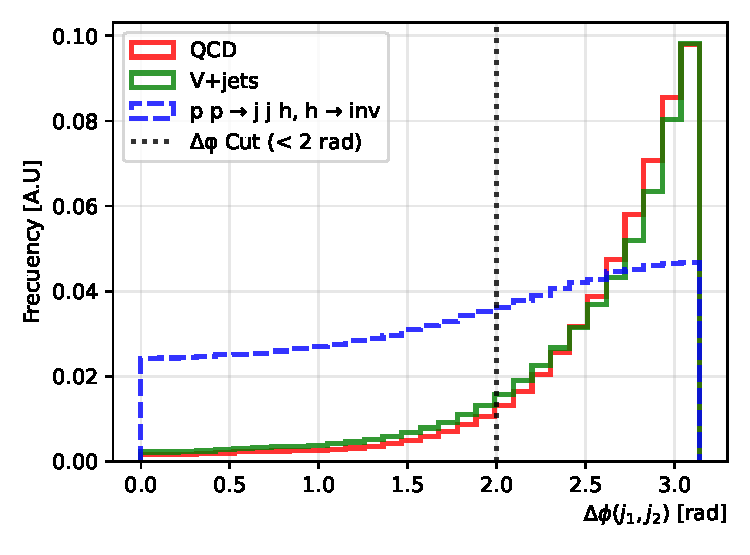
\includegraphics[width=\textwidth]{../Images/delta_phi_comparison.pdf}
\end{frame}

\begin{frame}{The Higgs-to-invisible decay left a High-MET signature}
    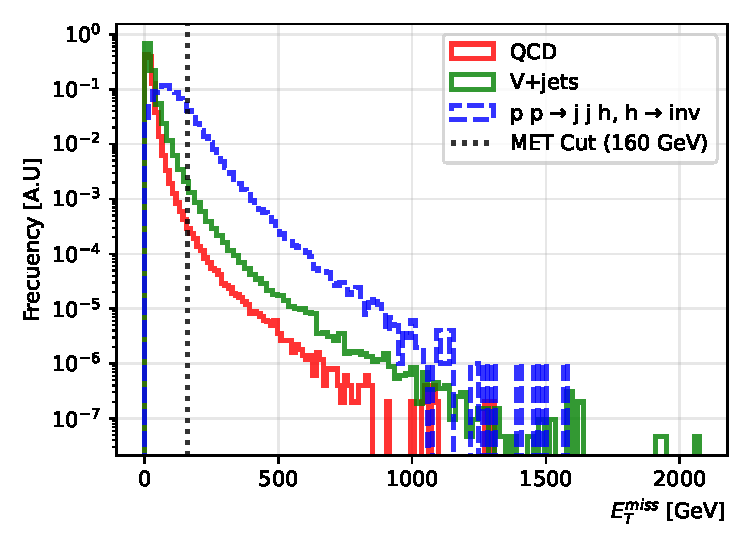
\includegraphics[width=\textwidth]{../Images/met_comparison.pdf}
\end{frame}

\begin{frame}{VBF Jets have a large invariant mass}
    $$
    m_{jj} = \sqrt{2 p_{T,1} p_{T,2} \left( \cosh(\Delta\eta) - \cos(\Delta\phi) \right)}
    \approx \sqrt{2 p_{T,1} p_{T,2} \cosh(\Delta\eta)}
    $$
    \begin{minipage}{0.9\textwidth}
        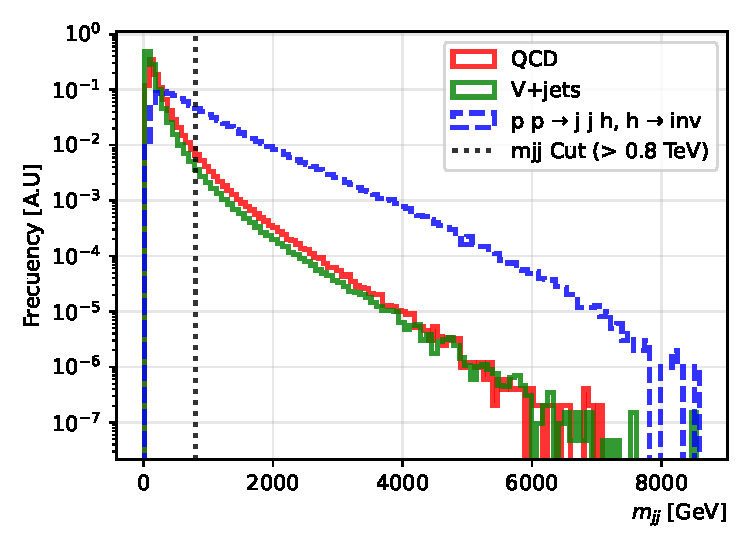
\includegraphics[width=\textwidth]{../Images/dijet_mass_comparison.pdf}
    \end{minipage}
\end{frame}




\begin{frame}{All the cuts suppres the background}
    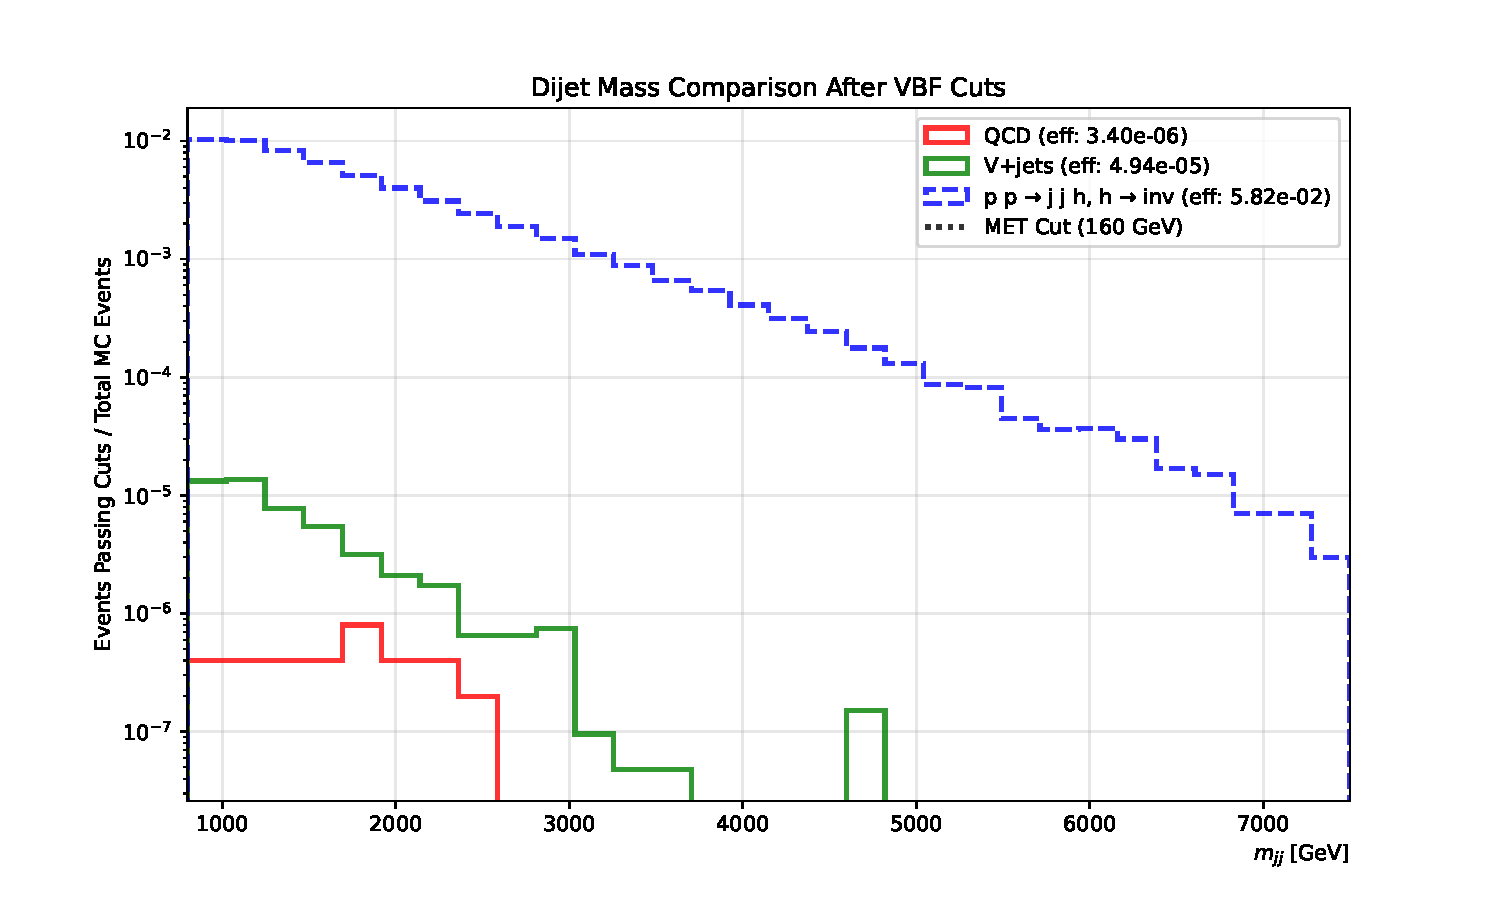
\includegraphics[width=.95\textwidth]{../Images/met_comparison_after_vbf_cuts.pdf}
\end{frame}


\section{Results and Projections}
\begin{frame}{Higgs-Portal Dark Matter Models}
    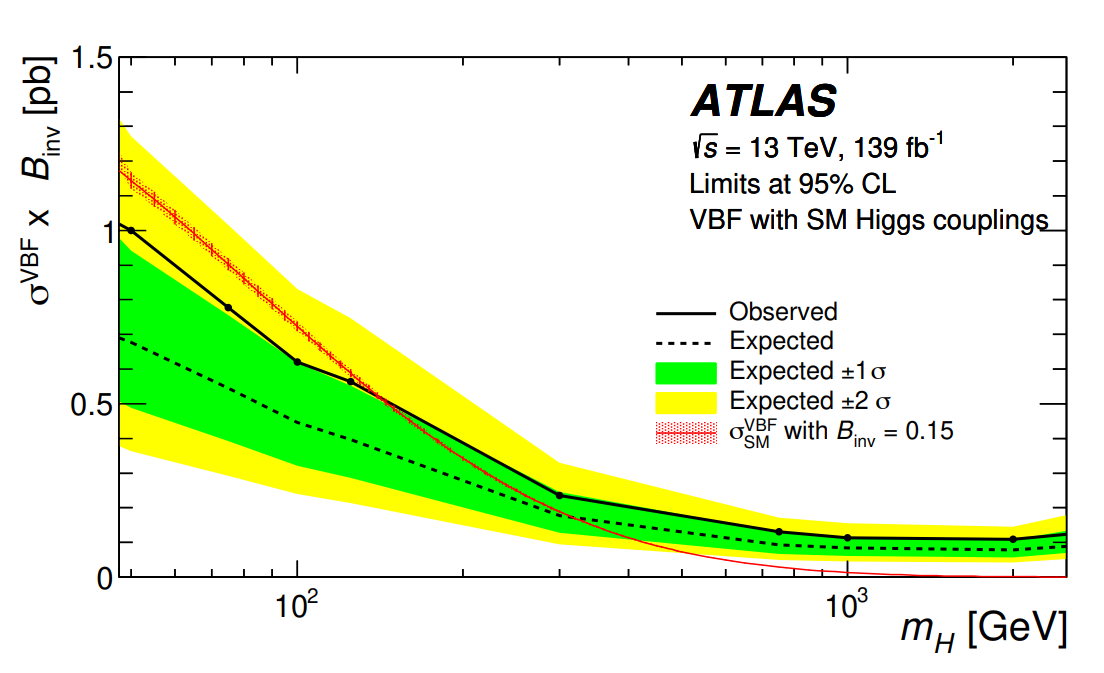
\includegraphics[width=\textwidth]{../Images/Altas_Result.png}
    $$
        BR(H \to \text{inv}) < 0.145 \quad \text{(ATLAS, 2019, 95\% CL)}
    $$
\end{frame}


\begin{frame}{Statistical Significance}
    The statistical significance is 
    \begin{equation}
        \kappa = \frac{\Braket{t}_{B} - \Braket{t}_{S+B}}{\sigma_{S+B}}
    \end{equation}
    where the optimal statistical test is $t=-2\ln \frac{\mathcal{L}(n|S+B)}{\mathcal{L}(n|B)}$, with $n$ the number expected of events in each hypothesis, $\mathcal{L}$ the likelihood function for $N$ a independet Poissonic distribution. so
    \begin{equation}
        \kappa = \frac{\sum_i s_i w_i}{\sqrt{\sum_i (s_i + b_i + \delta_{sys}^2)^2 w_i^2}}
    \end{equation}
    where $s_i$ and $b_i$ are the signal and background events in the $i$-th bin, $w_i\sim \ln (1+\frac{s_i}{b_i})$ is the weight of the $i$-th bin, and $\delta_{sys}$ is the systematic uncertainty in the background estimation.

    Hypothesis with a significance of $\kappa \leq 1.69\sigma$ will be excluded in searches with a 95\% confidence level (CL).
\end{frame}


\begin{frame}{Statistical Significance}
    

    The contribution to the number of events is of the form $N_i = \sigma_i \cdot \mathcal{L} \cdot \epsilon_i$, where $\sigma_i$ is the cross section of the process, $\mathcal{L}$ is the integrated luminosity, and $\epsilon_i$ is the efficiency of the selection cuts in the $i$-th bin.

    To improve the sensitivity of the search, 
    \begin{equation}
        \kappa = \frac{\sum_i s_i w_i}{\sqrt{\sum_i (s_i + b_i + \delta_{sys}^2)^2 w_i^2}}
        =\frac{\sum_i \textcolor{orange}{\sigma_{s_i}} \textcolor{red}{\epsilon_{s_i}} \textcolor{purple}{w_i}}{\sqrt{\sum_i (\textcolor{orange}{\sigma_{s_i}}\textcolor{red}{\epsilon_{s_i}} + \sigma_{b_i}\textcolor{red}{\epsilon_{b_i}} + \textcolor{green}{\delta_{\sigma_{sys}}^2})^2 \textcolor{purple}{w_i}^2}}\sqrt{\textcolor{blue}{\mathcal L}}
    \end{equation}
    We can
    \begin{itemize}
        \item \textcolor{blue}{Increase the integrated luminosity $\mathcal{L}$.}
        \item \textcolor{red}{Optimize the selection cuts to increase the efficiency $\epsilon_i$ of the signal and reduce the background.}
        \item \textcolor{orange}{increase the cross section $\sigma_i$ of the signal process increasing the center-of-mass energy $\sqrt{s}$ of the collisions.}
        \item Add information from the correlation between bins of the histogram.
        \item \textcolor{purple}{Select a observable that optimize the form of the $w_i$ weights (e.g. a BDT classifier).}
        \item \textcolor{green}{Reduce the systematic uncertainties $\delta_{sys}$ in the background estimation.}
    \end{itemize}
    
\end{frame}


\begin{frame}{Projections on the Higgs-to-invisible decay}
    So, taking $\kappa=1.69$ we have

    \begin{equation}
         \frac{\sum_i \sigma_{s_i} \epsilon_{s_i} w_i}{\sqrt{\sum_i (\sigma_{s_i}\epsilon_{s_i} + \sigma_{b_i}\epsilon_{b_i} + \delta_{\sigma_{sys}}^2)^2 w_i^2}}
         =
         \frac{\sum_i \sigma_{s_i}^{\text{VBF}}(\text{BR}) \epsilon_{s_i} w_i}{\sqrt{\sum_i (\sigma_{s_i}^{\text{VBF}}(\text{BR}) + \sigma_{b_i}\epsilon_{b_i} + \delta_{\sigma_{sys}}^2)^2 w_i^2}}
         = \frac{1.69}{\sqrt{\mathcal L}}
    \end{equation}

    In a conservative approach if we assume that the efficiencies and systematic uncertainties are constant, for future searches the limit on the Branching Ratio (BR) will scale inversely with the integrated luminosity $\mathcal{L}$. 
    \begin{itemize}
        \item The current limit, at $139 \text{ fb}^{-1}$ on the Higgs-to-invisible decay is $\text{BR}(H \to \text{inv}) < 0.145$.\pause
        \item Today the luminosity in ATLAS and CMS are arround 300~fb$^{-1}$ by the end of Run~3. So, in the near future we expect that LHC reach a sensitivity of $\text{BR}(H \to \text{inv}) < 0.08$.\pause
        \item With the HL-LHC, the promised integrated luminosity is 3 ab$^{-1}$, which will allow us to improve the sensitivity to $\text{BR}(H \to \text{inv}) < 0.008 \sim \mathcal{O}(10^{-2})$.\pause
        \item For FCC, the expected integrated luminosity is 30 ab$^{-1}$, which will allow us to improve the sensitivity to $\text{BR}(H \to \text{inv}) < \mathcal{O}(10^{-3})$.
    \end{itemize}
    
\end{frame}

\section{Interpretation on Higgs Portals}

\begin{frame}{Higgs Portals}
    We assume the minimal Higgs portal setup with singlet DM of spin 0 or spin 1/2. In that follows, we consider these options separately and allow for both CP-even and CP-odd couplings of the DM fermion to the Higgs field. The Lagrangian reads
    $$
        \begin{aligned}
        \mathcal{L}_{h s} & =\frac{\lambda_{h s}}{2} \mathcal{H}^{\dagger} \mathcal{H} S S \\
        \mathcal{L}_{h \chi} & =\frac{1}{\Lambda} \mathcal{H}^{\dagger} \mathcal{H} \bar{\chi} \chi, \quad \mathcal{L}_{h \chi}^{\gamma_5}=\frac{1}{\Lambda_5} \mathcal{H}^{\dagger} \mathcal{H} \bar{\chi} i \gamma_5 \chi,
        \end{aligned}
    $$
    where $\mathcal{H}$ is the Higgs doublet, $S$ is a real scalar singlet with mass $m_s$, and $\chi$ is a Dirac fermion with mass $m_\chi$. 
    \begin{gather*}
        \Gamma(h \rightarrow S S)=\frac{\lambda_{h s}^2 v^2}{32 \pi m_h} \sqrt{1-\frac{4 m_s^2}{m_h^2}} \\
        \Gamma_{\text{CP-even}}(h \rightarrow \chi \chi)=\frac{m_h}{4 \pi} \frac{v^2}{\Lambda^2}\left(1-\frac{4 m_\chi^2}{m_h^2}\right)^{3 / 2}; \quad 
        \Gamma_{\text{CP-odd}}(h \rightarrow \chi \chi)=\frac{m_h}{4 \pi} \frac{v^2}{\Lambda_5^2}\left(1-\frac{4 m_\chi^2}{m_h^2}\right)^{1 / 2}
    \end{gather*}
    These states are assumed to be stable adn thus can be considered as DM candidates. In the fermionic case, the couplings are non-renormalizable and thus are understood as effective operators with $\Lambda$ and $\Lambda_5$ being the cut-off scales. 
\end{frame}

\begin{frame}{$\Gamma(h \rightarrow S S)=\frac{\lambda_{h s}^2 v^2}{32 \pi m_h} \sqrt{1-\frac{4 m_s^2}{m_h^2}}$}
    \begin{center}
        \includegraphics[width=.9\textwidth]{../Images/Portal_to_Scalar.pdf}
    \end{center}
\end{frame}
\begin{frame}{$\Gamma_{\text{CP-even}}(h \rightarrow \chi \chi)=\frac{m_h}{4 \pi} \frac{v^2}{\Lambda^2}\left(1-\frac{4 m_\chi^2}{m_h^2}\right)^{3 / 2}; $}
    \begin{center}
        \includegraphics[width=.9\textwidth]{../Images/Portal_to_cp_even_fermion.pdf}
    \end{center}
\end{frame}

\begin{frame}{$\Gamma_{\text{CP-odd}}(h \rightarrow \chi \chi)=\frac{m_h}{4 \pi} \frac{v^2}{\Lambda_5^2}\left(1-\frac{4 m_\chi^2}{m_h^2}\right)^{1 / 2}$}
    \begin{center}
        \includegraphics[width=.9\textwidth]{../Images/Portal_to_cp_odd_fermion.pdf}
    \end{center}
\end{frame}

\begin{frame}{Example: Scalar-Fermion Z4 model}
    $$
    \mathcal{L}=\frac{1}{2} \mu_S^2 S^2+\lambda_S S^4+\frac{1}{2} \lambda_{S H}|H|^2 S^2+M_\psi \bar{\psi} \psi+\frac{1}{2}\left[y_s \overline{\psi^c} \psi+y_p \overline{\psi^c} \gamma_5 \psi+\text { h.c. }\right] S,
    $$

    In the $M_S < M_\psi$ regime, 
    \begin{center}
        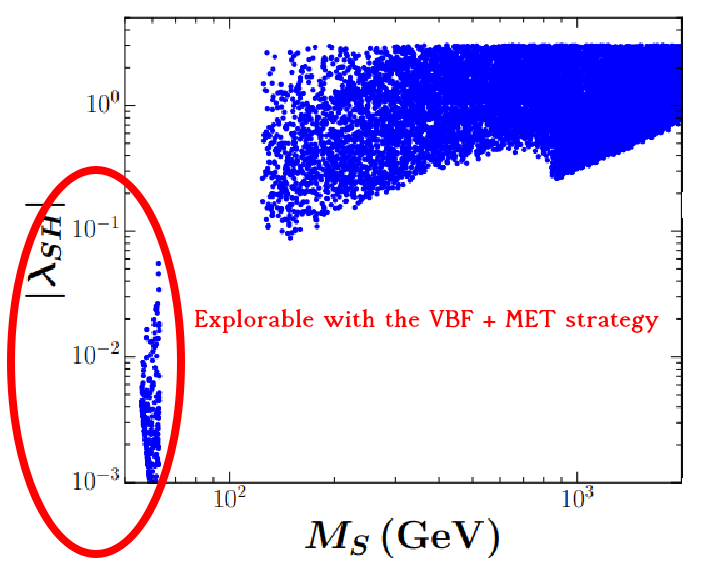
\includegraphics[width=.6\textwidth]{../Images/Z4_Example.png}
    \end{center}
    \cite{Yaguna:2021rds}
\end{frame}

\begin{frame}{Summary}
    \begin{itemize}
        \item We investigated Higgs-portal dark matter models using VBF + MET signatures at the LHC
        \item Performed Monte Carlo simulations with MadGraph5\_aMC@NLO to compute cross sections for VBF Higgs production with invisible decays
        \item Analyzed kinematic variables showing VBF jets are:
        \begin{itemize}
            \item High-$p_T$ and forward
            \item In opposite hemispheres with large $\Delta\eta$ separation
            \item Associated with high missing transverse energy
        \end{itemize}
        \item Current experimental limit: $\text{BR}(H \to \text{inv}) < 0.145$ (ATLAS, 139 fb$^{-1}$)
        \item Projected sensitivity improvements:
        \begin{itemize}
            \item Run 3 (300 fb$^{-1}$): $\text{BR}(H \to \text{inv}) < 0.08$
            \item HL-LHC (3 ab$^{-1}$): $\text{BR}(H \to \text{inv}) < 0.008$
            \item FCC (30 ab$^{-1}$): $\text{BR}(H \to \text{inv}) < \mathcal{O}(10^{-3})$
        \end{itemize}
        \item Provided exclusion contours for scalar and fermionic DM in the mass-coupling parameter space
    \end{itemize}
\end{frame}

\begin{frame}
    \centering
    \Huge Thank you for your attention!
    \vfill
    \Large Questions?
\end{frame}
\end{document}